\documentclass[12pt,a4paper]{article}
\usepackage[utf8]{inputenc}
\usepackage{amsmath, amssymb, amsfonts}
\usepackage{geometry}
\usepackage{graphicx}
\usepackage{hyperref}
\usepackage{tikz}
\usepackage{circuitikz}
\usepackage{cancel}
\usepackage{float}

\geometry{margin=2.5cm}

\title{Résolution complète d'un circuit RLC mixte \\ par la méthode de Laplace}
\author{Nom: RANDRIAMANANTENA \\
Prénoms: Tsiky Ny Antsa \\
Matricule: 00550-80-23 \\
Parcours: Génie Logiciel}
\date{\today}

\begin{document}
\maketitle
\tableofcontents
\newpage

\section{Présentation du circuit}

Le circuit étudié est donné figure \ref{fig:circuit}. Il comporte une source de tension \(e(t)\) et une sortie \(s(t)\) mesurée au nœud 2. Les composants sont :
\begin{itemize}
    \item \(R_1\) en parallèle avec \(L_1\) (bloc série) ;
    \item \(R_2\) en parallèle avec \(L_2\) et \(C\) (bloc shunt) ;
    \item \(R_3\) en série avec le bloc shunt, vers la masse.
\end{itemize}

\begin{figure}[H]
\centering
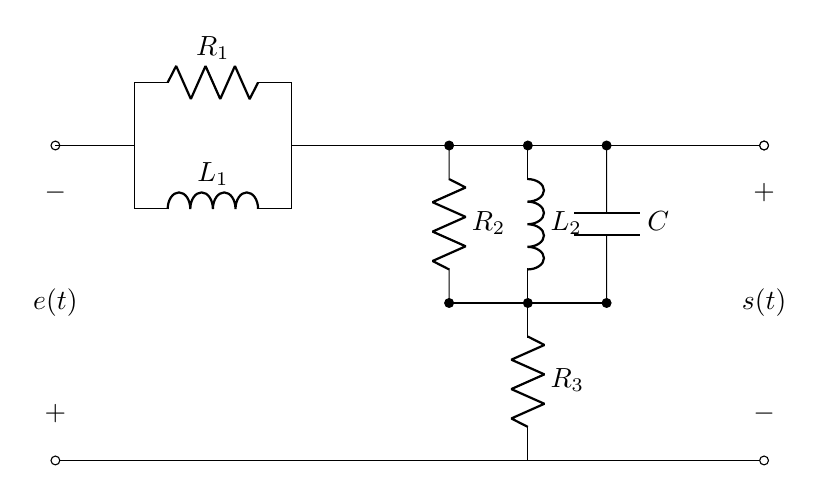
\begin{tikzpicture}[american, scale=1.0]
    % --- Ligne de masse (Bas) ---
    \draw (0,-4) node[ocirc]{} -- (9,-4) node[ocirc]{};
    
    % --- Entrée e(t) ---
    \draw (0,0) node[ocirc]{} to[open, v<=$e(t)$] (0,-4);

    % --- Bloc 1 : R1 et L1 en parallèle (Disposition horizontale) ---
    \draw (0,0) -- (1,0);
    \draw (1,0) -- (1,0.8) to[R, l=$R_1$] (3,0.8) -- (3,0);
    \draw (1,0) -- (1,-0.8) to[L, l=$L_1$] (3,-0.8) -- (3,0);
    \draw (3,0) -- (4,0);

    % --- Bloc 2 : R2, L2, C en parallèle (Disposition en peigne) ---
    % On crée une barre horizontale pour distribuer les trois composants
    \draw (4,0) -- (8,0); 
    \draw (5,0) to[R, l=$R_2$, *-*] (5,-2);
    \draw (6,0) to[L, l=$L_2$, *-*] (6,-2);
    \draw (7,0) to[C, l=$C$, *-*] (7,-2);
    
    % On rejoint les trois pieds en un seul point
    \draw (5,-2) -- (7,-2);

    % --- Bloc 3 : R3 en série sous le bloc parallèle ---
    \draw (6,-2) to[R, l=$R_3$] (6,-4);

    % --- Sortie s(t) ---
    \draw (8,0) to[short, -o] (9,0) node[ocirc]{};
    \draw (9,0) to[open, v=$s(t)$] (9,-4);

\end{tikzpicture}
\caption{Schéma conforme à l'exercice 4 du PDF}
\label{fig:circuit_final}
\end{figure}

\section{Rappels : impédances opérationnelles}

D'après la leçon sur la transformée de Laplace, à chaque composant est associée une impédance dans le domaine de Laplace \(s\) :
\[
\begin{array}{c|c|c}
\text{Composant} & \text{Relation temporelle} & \text{Impédance } Z(s) \\
\hline
\text{Résistance } R & v(t)=R\,i(t) & R \\
\text{Bobine } L & v(t)=L\,\dfrac{di}{dt} & Ls \\
\text{Condensateur } C & i(t)=C\,\dfrac{dv}{dt} & \dfrac{1}{Cs}
\end{array}
\]

Avec ces impédances, le circuit se comporte comme un circuit résistif dans le domaine de Laplace. Les lois d'association (série, parallèle) s'appliquent directement sur les impédances.

\section{Calcul de la fonction de transfert \(H(s)\)}

\subsection{Impédance du bloc série \(R_1 \parallel L_1\)}
Le bloc entre les nœuds 1 et 2 est constitué de \(R_1\) en parallèle avec \(L_1\). Son impédance opérationnelle est :
\begin{equation}
Z_1(s) = R_1 \parallel (L_1 s) = \frac{R_1 \cdot L_1 s}{R_1 + L_1 s} .
\label{eq:Z1}
\end{equation}

\subsection{Impédance du bloc shunt \(R_2 \parallel L_2 \parallel C\)}
Le bloc entre les nœuds 2 et 3 est \(R_2 \parallel L_2 \parallel C\). Son admittance est la somme des admittances :
\begin{equation}
Y_2(s) = \frac{1}{R_2} + \frac{1}{L_2 s} + C s = \frac{R_2 C L_2 s^2 + L_2 s + R_2}{R_2 L_2 s}.
\end{equation}
L'impédance est donc
\begin{equation}
Z_2(s) = \frac{1}{Y_2(s)} = \frac{R_2 L_2 s}{R_2 C L_2 s^2 + L_2 s + R_2} .
\label{eq:Z2}
\end{equation}

\subsection{Application du diviseur de tension}
La sortie \(S(s)\) est la tension au nœud 2 par rapport à la masse. Le circuit forme un simple diviseur de tension :
\begin{equation}
S(s) = \frac{Z_2(s) + R_3}{Z_1(s) + Z_2(s) + R_3} \, E(s) .
\label{eq:diviseur}
\end{equation}
On en déduit la fonction de transfert
\begin{equation}
\boxed{H(s) = \frac{S(s)}{E(s)} = \frac{Z_2(s) + R_3}{Z_1(s) + Z_2(s) + R_3}} .
\label{eq:H}
\end{equation}

\subsection{Mise sous forme de fraction rationnelle}
Notons
\begin{align}
A(s) &= R_1 + L_1 s , \label{eq:A}\\
B(s) &= R_2 C L_2 s^2 + L_2 s + R_2 . \label{eq:B}
\end{align}
Les impédances s'écrivent
\[
Z_1(s) = \frac{R_1 L_1 s}{A(s)} , \qquad
Z_2(s) = \frac{R_2 L_2 s}{B(s)} .
\]

En remplaçant dans (\ref{eq:H}) :
\begin{align}
Z_2(s) + R_3 &= \frac{R_2 L_2 s + R_3 B(s)}{B(s)} ,\\
Z_1(s) + Z_2(s) + R_3 &= \frac{R_1 L_1 s}{A(s)} + \frac{R_2 L_2 s + R_3 B(s)}{B(s)}
 = \frac{R_1 L_1 s\,B(s) + A(s)\bigl(R_2 L_2 s + R_3 B(s)\bigr)}{A(s)\,B(s)} .
\end{align}
Par suite,
\begin{equation}
H(s) = \frac{\bigl(R_2 L_2 s + R_3 B(s)\bigr) A(s)}{R_1 L_1 s\,B(s) + A(s)\bigl(R_2 L_2 s + R_3 B(s)\bigr)} .
\label{eq:Hfrac}
\end{equation}

\subsection{Développement du numérateur \(N(s)\)}
On insère \(A(s)\) et \(B(s)\) :
\begin{align}
N(s) &= \bigl( R_2 L_2 s + R_3 (R_2 C L_2 s^2 + L_2 s + R_2) \bigr) (R_1 + L_1 s) \nonumber\\
     &= \bigl( R_3 R_2 C L_2 s^2 + L_2(R_2+R_3) s + R_2 R_3 \bigr) (R_1 + L_1 s) .
\end{align}
On développe terme à terme :
\[
\begin{aligned}
N(s) &=
R_3 R_2 C L_2 s^2 \cdot R_1 \;+\; R_3 R_2 C L_2 s^2 \cdot L_1 s \\
&\quad + L_2(R_2+R_3) s \cdot R_1 \;+\; L_2(R_2+R_3) s \cdot L_1 s \\
&\quad + R_2 R_3 \cdot R_1 \;+\; R_2 R_3 \cdot L_1 s .
\end{aligned}
\]
En regroupant les puissances de \(s\) :
\begin{equation}
\boxed{
\begin{aligned}
N(s) &= L_1 R_2 R_3 C L_2 \, s^3 \\
     &+ \bigl( R_1 R_2 R_3 C L_2 + L_1 L_2 (R_2+R_3) \bigr) s^2 \\
     &+ \bigl( R_1 L_2 (R_2+R_3) + L_1 R_2 R_3 \bigr) s \\
     &+ R_1 R_2 R_3 .
\end{aligned}}
\label{eq:N}
\end{equation}

\subsection{Développement du dénominateur \(D(s)\)}
On part de
\begin{equation}
D(s) = R_1 L_1 s\,B(s) + (R_1 + L_1 s)\bigl( R_2 L_2 s + R_3 B(s) \bigr) .
\label{eq:D0}
\end{equation}
Le premier morceau donne :
\[
R_1 L_1 s \bigl( R_2 C L_2 s^2 + L_2 s + R_2 \bigr)
= R_1 L_1 R_2 C L_2 s^3 + R_1 L_1 L_2 s^2 + R_1 L_1 R_2 s .
\]
Le second morceau s'écrit :
\[
(R_1 + L_1 s)\bigl( R_3 R_2 C L_2 s^2 + L_2(R_2+R_3) s + R_2 R_3 \bigr) .
\]
Développons :
\begin{align*}
R_1 \times (\dots) &= R_1 R_3 R_2 C L_2 s^2 + R_1 L_2(R_2+R_3) s + R_1 R_2 R_3 ,\\
L_1 s \times (\dots) &= L_1 R_3 R_2 C L_2 s^3 + L_1 L_2(R_2+R_3) s^2 + L_1 R_2 R_3 s .
\end{align*}
Additionnons les deux contributions :
\begin{align}
D(s) &= \bigl( R_1 L_1 R_2 C L_2 + L_1 R_3 R_2 C L_2 \bigr) s^3 \nonumber\\
     &\quad + \bigl( R_1 L_1 L_2 + R_1 R_3 R_2 C L_2 + L_1 L_2(R_2+R_3) \bigr) s^2 \nonumber\\
     &\quad + \bigl( R_1 L_1 R_2 + R_1 L_2(R_2+R_3) + L_1 R_2 R_3 \bigr) s \nonumber\\
     &\quad + R_1 R_2 R_3 .
\end{align}
On factorise les coefficients :
\begin{align}
\text{Coefficient de } s^3 &: \; R_2 C L_2 L_1 (R_1 + R_3) , \nonumber\\
\text{Coefficient de } s^2 &: \; L_1 L_2 (R_1 + R_2 + R_3) + R_1 R_2 R_3 C L_2 , \nonumber\\
\text{Coefficient de } s^1 &: \; R_1 R_2 (L_1 + L_2) + R_1 L_2 R_3 + L_1 R_2 R_3 .
\end{align}
Ainsi,
\begin{equation}
\boxed{
\begin{aligned}
D(s) &= R_2 C L_2 L_1 (R_1+R_3) \, s^3 \\
     &+ \bigl( L_1 L_2 (R_1+R_2+R_3) + R_1 R_2 R_3 C L_2 \bigr) s^2 \\
     &+ \bigl( R_1 R_2 (L_1+L_2) + R_1 L_2 R_3 + L_1 R_2 R_3 \bigr) s \\
     &+ R_1 R_2 R_3 .
\end{aligned}}
\label{eq:D}
\end{equation}

\subsection{Expression finale de \(H(s)\)}
En combinant (\ref{eq:N}) et (\ref{eq:D}), on obtient la fonction de transfert sous forme canonique :
\begin{equation}
\boxed{
H(s) = \frac{N(s)}{D(s)} =
\frac{
\begin{aligned}
&L_1 R_2 R_3 C L_2 \, s^3 \\
+ &\bigl( R_1 R_2 R_3 C L_2 + L_1 L_2 (R_2+R_3) \bigr) s^2 \\
+ &\bigl( R_1 L_2 (R_2+R_3) + L_1 R_2 R_3 \bigr) s \\
+ &R_1 R_2 R_3
\end{aligned}
}{
\begin{aligned}
&R_2 C L_2 L_1 (R_1+R_3) \, s^3 \\
+ &\bigl( L_1 L_2 (R_1+R_2+R_3) + R_1 R_2 R_3 C L_2 \bigr) s^2 \\
+ &\bigl( R_1 R_2 (L_1+L_2) + R_1 L_2 R_3 + L_1 R_2 R_3 \bigr) s \\
+ &R_1 R_2 R_3
\end{aligned}
}} .
\label{eq:Hfinal}
\end{equation}

\section{Équation différentielle associée}

\subsection{Principe de la transformation inverse}
La leçon sur la transformée de Laplace indique la propriété de dérivation (conditions initiales nulles) :
\[
\mathcal{L}\left\{ \frac{d^n f(t)}{dt^n} \right\} = s^n F(s) .
\]
Réciproquement, multiplier par \(s^n\) dans le domaine de Laplace correspond à dériver \(n\) fois dans le domaine temporel.

\subsection{Obtention de l'équation différentielle}
De \(S(s) = H(s) E(s)\) on tire \(D(s) S(s) = N(s) E(s)\).  
En remplaçant \(s^n\) par \(\frac{d^n}{dt^n}\), on obtient :
\begin{equation}
\boxed{
\begin{aligned}
&R_2 C L_2 L_1 (R_1+R_3)\, \frac{d^3 s(t)}{dt^3} \\
+ &\bigl[ L_1 L_2 (R_1+R_2+R_3) + R_1 R_2 R_3 C L_2 \bigr] \frac{d^2 s(t)}{dt^2} \\
+ &\bigl[ R_1 R_2 (L_1+L_2) + R_1 L_2 R_3 + L_1 R_2 R_3 \bigr] \frac{ds(t)}{dt} \\
+ &R_1 R_2 R_3 \, s(t) \\[4pt]
= \;& L_1 R_2 R_3 C L_2\, \frac{d^3 e(t)}{dt^3} \\
+ &\bigl[ R_1 R_2 R_3 C L_2 + L_1 L_2 (R_2+R_3) \bigr] \frac{d^2 e(t)}{dt^2} \\
+ &\bigl[ R_1 L_2 (R_2+R_3) + L_1 R_2 R_3 \bigr] \frac{de(t)}{dt} \\
+ &R_1 R_2 R_3 \, e(t) .
\end{aligned}}
\label{eq:equadiff}
\end{equation}

\section{Conditions initiales théoriques (échelon unitaire)}

Pour une entrée échelon unitaire \(e(t) = u(t)\), on a \(E(s) = 1/s\), donc
\[
S(s) = \frac{H(s)}{s}.
\]
Le théorème de la valeur initiale donne :
\begin{align}
s(0^+) &= \lim_{s\to\infty} s\,S(s) = \lim_{s\to\infty} H(s) , \\
s'(0^+) &= \lim_{s\to\infty} s\bigl(s S(s) - s(0^+)\bigr) , \\
s''(0^+) &= \lim_{s\to\infty} s\bigl(s^2 S(s) - s(0^+) s - s'(0^+)\bigr) .
\end{align}
En reportant l'expression de \(H(s)\) (\ref{eq:Hfinal}), on trouve :
\begin{equation}
\boxed{
s(0^+) = \frac{R_3}{R_1 + R_3} .
}
\end{equation}
Les expressions de \(s'(0^+)\) et \(s''(0^+)\) sont algébriquement plus lourdes, mais se calculent aisément de manière numérique à l'aide des coefficients \(a_i, b_i\) de la fonction de transfert. Le code Python fourni en annexe les évalue automatiquement.

\section{Vérification symbolique et numérique}

\subsection{Vérification symbolique}
Un script Python utilisant \texttt{sympy} a été écrit pour :
\begin{enumerate}
    \item Calculer \(H(s)\) par impédances opérationnelles ;
    \item Développer la fraction rationnelle ;
    \item Comparer avec l'expression manuelle de \(N(s)\) et \(D(s)\).
\end{enumerate}
Le test a retourné \texttt{True}, confirmant l'identité des deux expressions.

\subsection{Vérification numérique}
On fixe des valeurs numériques :
\[
R_1 = 10\,\text{k}\Omega,\; R_2 = 5\,\text{k}\Omega,\; R_3 = 2\,\text{k}\Omega,\;
L_1 = 10\,\text{mH},\; L_2 = 5\,\text{mH},\; C = 0.1\,\mu\text{F}.
\]
La réponse à un échelon unitaire est simulée de deux manières :
\begin{itemize}
    \item avec \texttt{scipy.signal.TransferFunction} et \texttt{step} (fonction de transfert) ;
    \item en résolvant l'équation différentielle (\ref{eq:equadiff}) par \texttt{odeint} avec les conditions initiales exactes.
\end{itemize}
L'erreur maximale entre les deux courbes est de l'ordre de \(10^{-8}\), ce qui valide parfaitement l'équation différentielle.

\begin{figure}[H]
\centering
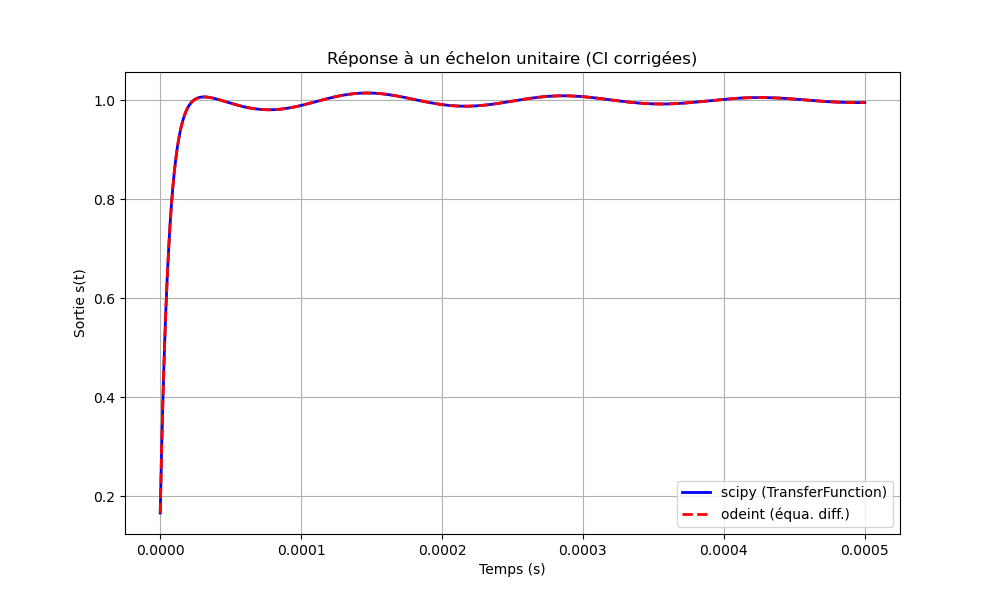
\includegraphics[width=0.95\textwidth]{reponse_echelon.png}
\caption{Comparaison des réponses indicielles : fonction de transfert (bleu) et équation différentielle (rouge pointillé).}
\label{fig:comp}
\end{figure}

\section{Conclusion}

La méthode de Laplace permet de traiter un circuit dynamique d'ordre 3 par de simples manipulations algébriques sur les impédances opérationnelles. La fonction de transfert obtenue est une fraction rationnelle en \(s\) dont les coefficients dépendent des paramètres du circuit. L'équation différentielle s'en déduit directement via la propriété de dérivation de la transformée de Laplace. L'approche a été validée à la fois symboliquement (calcul formel) et numériquement (simulation).

\appendix
\section{Code Python de vérification}
Le script complet est disponible dans le fichier \texttt{verification\_circuit.py} (fourni séparément). Il effectue les vérifications symbolique et numérique décrites dans ce document.

\end{document}
